%!TEX root = main.tex

\section{System Measurement}
\label{sec:system-measurement}

In this section, we use the TCP traces described above to measure our crowdsourced live video system. In Section~\ref{sub:upload-analysis} we will analyze the TCP upload flows, which transfer video data from camera to front-end server. In Section~\ref{sub:download-analysis} we will analyze the TCP download flows, which distribute video data from front-end server to viewers. And in Section~\ref{sub:relationship-analysis} we will analyze the relationship between the upload and download flows and try to figure out how the upload performance impacts the whole system performance.

\subsection{Analysis of TCP upload flows}
\label{sub:upload-analysis}

Video sharing users upload video to front-end server once they produce frames. The fluency of upload video directly impact the Quality of Experience of video viewing. Two factors may influence the upload process: one is the interval of frame producing process and the other is the delay by the network. We define \emph{TCP stall} as an event where the duration between two consecutive packets received/sent by the server is larger than $\min(\tau\cdot\text{SRTT}, \text{RTO})$. Parameter $\tau$ is set to 2 in this work as the TCP endpoint could at least receive or send one packet during $2RTT$ in the ideal condition. As the front-end server (where we collected the data) is the receiver in the upload flow, we can only measure the 3-Way HandShake (3WHS) RTT during which servers send a SYN packet and receive the corresponding acknowledgment. Thus, we use the RTT in 3WHS as the \text{SRTT} for this flow. 

The front-end server, as a receiver in the upload flow, may receive a series of disordered packets, in which the packets in the hole (\ie not received in sequential order) may be reordered by the network, or retransmitted because the previously transmitted segment is dropped. The front-end server could not distinguish whether the disordered packet is a packet reordering or packet retransmission. When a stall happens, receivers may have received a series of disordered packets, or sequential packets. We further distinguish the stalls by labeling the former as \emph{reordering stall} and the latter as \emph{normal stall}. When not receiving any video data from the camera, front-end server will send keep-alive packets, per in 5 seconds, to make the connection open. We find that all the stall time accounts for 31.6\% of all the completion time in the upload flows. Among these stalls, normal stall contributes 93.5\% of stall time, reordering stall contributes 1.3\% of stall time, keep-alive stall accounts for 5.2\% of stall time. It means that packet loss or reordering is not the main factor of network stalls. However, the interval of frame produced process is the main factor that influence the upload flow. That can also be confirmed by the fact that the median throughput of upload flows is 60KB/s, much smaller than the available upload bandwidth.

\iffalse
 The percentage of different stall time is shown in Table~\ref{tbl:upload-stall}.
\begin{table}[ht]
\tablefontsize
\renewcommand{\arraystretch}{\assize}
 \setlength{\tabcolsep}{3pt}
\caption{Percentage of different stall in upload flows.}
\centering
\begin{tabular}{c|c}
	\toprule
	 type & percentage(\%) \\
	\hline
	normal & 93.5 \\
	\hline
	reorder & 1.3 \\
	\hline
	keep alive & 5.2 \\
	\bottomrule
\end{tabular}
\label{tbl:upload-stall}
\termspace
\end{table} 
From Table~\ref{tbl:upload-stall}, we can see that 93.5\% stall is normal stall while the reorder stall is just 1.3\%. 
\fi

We define reordering rate as the ratio of packets which do not arrive in order to all data packets. We find that the overall reordering rate is about 1\% and among those disordered packets, 6\% of them suffer from timeout reordering, which means the interval between two disordered packets is larger than 0.2 second (\ie the minimum RTO set in Linux kernel). Although packet loss or reordering happens rarely, once it happens, it will significantly impact the performance of upload flows. We find that packet reordering strongly correlates with the size of upload flow, especially when the reordering rate becomes large. Table~\ref{tbl:reorder-rate-influence} shows the impact of reordering rate on upload flow size. When the reordering rate becomes larger, the performance of upload flows degrades dramatically.

% We further find that the total frame's reorder rate is 1\% and among the reorder packets 6\% suffer from timeout reorder. If the packet in upload flow is lost and can not be recovered by fast retransmit, the front-end server will receive a timeout reorder packet. We define the reorder packet as timeout reorder packet if the interval between the reorder packet and the last send-in data is larger than 0.2 second(the minimum RTO in linux kernel). Although packet loss or reordering is not the main factor that impacts the performance of upload flows, we find that packet reordering strongly correlates with the size of upload flow, especially when the reordering rate becomes large. Table~\ref{tbl:reorder-rate-influence} shows the impact of reordering rate on upload flow size. When the reordering rate becomes larger, the performance of upload flows degrades dramatically. 

% Although the packet loss or reorder is not the main factor that influences the upload flow rate, we find that packet reorder rate greatly influence the upload flow size, especially when the reorder rate becomes large. Table~\ref{tbl:reorder-rate-influence} shows the influence of reorder rate to upload flows. As reorder rate grows, the upload flows' flow rate, flow size and FCT(Flow Complete Time) become small. 

When the reordering rate is larger than 20\%, which means the network quality is very bad, the mean size of upload flows becomes 0.73MB, much smaller than the flow size (5.1MB) when the reordering rate is less than 10\%. The video sharing users also views the video that he or she uploads. If the upload network is bad and the reordering rate becomes high, video sharing user is likely to terminate the upload process. That is why the flow size suddenly drops when the reordering rate becomes large. 

\begin{table}[ht]
\tablefontsize
\renewcommand{\arraystretch}{\assize}
 \setlength{\tabcolsep}{3pt}
\caption{Impact of reordering rate on the performance of upload flows.}
\centering
\begin{tabular}{c|c|c|c}
	\toprule
	reordering rate & avg throughput & flow size & FCT \\
	\hline
	$<$10\% & 64KB/s & 5.1MB & 87.7s \\
	\hline
	10-20\% & 48KB/s & 4.7MB & 72.8s \\
	\hline
	$>$20\% & 17KB/s & 0.73MB & 60.7s \\
	\bottomrule
\end{tabular}
\label{tbl:reorder-rate-influence}
\termspace
\end{table}  

\subsection{Analysis of TCP download flows}
\label{sub:download-analysis}

To figure out what factors influence the download flows between front-end server and viewers, we analyze the stalls in the TCP download flow. The \emph{stall} in download flows is defined the same as in Section~\ref{sub:upload-analysis}. As the front-end server is the sender in the video viewing process, it could calculate RTT dynamically each time it receives acknowledgment of the transmitted data.

According to the position where each stall happens, we further classify these stalls into the following types. \emph{Timeout retrans} stalls are those caused by the timeout retransmissions. \emph{Resource constraint} stall happens when there is no data in the buffer to transmit and is often caused by that the camera does not upload data timely.%(the same as the normal stall in Section~\ref{sub:upload-analysis} \wu{Normal stall can also be triggered for other reasons, \eg zero receive window.}). 
\emph{Packet delay} stall is caused when the ACK packets are delayed, either by network or receiver. When a viewer does not have enough buffer to store the data it will reduce its receive window (rwnd) to zero, thus the front-end server can not send any data until the viewer enlarges its rwnd. Such a stall is defined as \emph{zero rwnd} stall. When there are no data to transmit, the front-end server will send a keep-alive packet every 5 seconds to prevent the connection to be terminated. Such a stall is labeled as \emph{keep alive} stall. In total the stall time occupies 35.2\% of the completion time of all download flows. Table~\ref{tbl:stall-download} shows the ratio of different stalls in terms of time in download flows.

\begin{table}[ht]
\tablefontsize
\renewcommand{\arraystretch}{\assize}
 \setlength{\tabcolsep}{3pt}
 \caption{Analysis for download flows}
 \centering
 \subtable[Ratio of different stalls in download flow.]{
\begin{tabular}{c|c}
	\toprule
	Stall Type & Percentage(\%)\\
	\hline
	resource constraint & 39.4   \\
	\hline
	packet delay & 8.2 \\
	\hline
	zero rwnd & 16.3 \\
	\hline
	keep alive & 10.1 \\
	\hline
	timeout retrans. & 22.8 \\
	\hline
	others & 1.5 \\
	\bottomrule
\end{tabular}
\label{tbl:stall-download}
}
\hspace{3em}
\subtable[Ratio of RTT over RTT\tsub{3WHS} when varying $in\_flight$.]{
\begin{tabular}{l|c}
	\toprule
	 $in\_flight$ & RTT/RTT\tsub{3WHS} \\
	\hline
	[0, 4KB) & 0.89 \\
	\hline
	[4KB, 8KB) & 1.08  \\
	\hline
	[8KB, 16KB) & 1.31  \\
	\hline
	[16KB, 32KB) & 1.38  \\
	\hline
	[32KB, 64KB) & 1.61 \\
	\hline
	[64KB, $\infty$) & 2.6  \\
	\bottomrule
\end{tabular}
\label{tbl:inflight-rtt}
}
\termspace
\label{tbl:download-flow-analysis}
\end{table}  

From Table~\ref{tbl:stall-download} we can see that the \emph{resource constraint} accounts for 39.4\% of all the download stall, the largest part amongst all, which is partially caused by the upload flows. In Section~\ref{sub:upload-analysis} we find that stalls account for 31.6\% of all upload flow time. As the camera stops sending data for a while, the front-end server does not have any data to send. About 16.3\% stalls belongs to \emph{zero rwnd} stall, which means the viewers' inability of receiving data will also greatly impact the performance of video viewing. \emph{Keep alive} stall accounts for 10.1\% of download stall time, indicating that there are users still waiting for some time to terminate the connection even when the video sharing user has stopped uploading video.
% \wu{Keep-alive stall is caused by that the data is unavailable for a long time (longer than 5 seconds), which does not mean the video upload flow has been terminated.}
22.8\% of stalls belong to \emph{timeout retrans}, which is caused by the network. In Section~\ref{sec:frame-analysis} we will further analyze the timeout retransmission stalls in detail.

\subsubsection{Analysis of RTT variation}
\label{sub:RTT}

RTT is an important factor that influences the flow rate. The flows with small RTT are more likely to get high flow rate. RTT is determined by two factors. One is the number of hops between two nodes which is controlled by the route algorithm. The other is the packets' cache time at the routers which is controlled both by the router buffer capacity and the volume of packets in the network. In the WAN, the route algorithm and router buffer capacity are out of the control of sever. The only way that the server can control the RTT is by controlling the packets that is sent to the network.

In table~\ref{tbl:inflight-rtt} we analyze the change of RTT when varying the $in\_flight$ size. Parameter $in\_flight$ represents the amount of data bytes sent already and not received yet by the viewers, which is defined as follows:
%\begin{footnotesize}
\begin{equation}
\label{eq:conserve}
\begin{aligned}
in\_flight = \enspace & packets\_out + retrans\_out \enspace - 
 (sacked\_out + lost\_out) \enspace ,
\end{aligned}
\end{equation}
%\end{footnotesize}
where $packets\_out$ is the data bytes between $snd\_una$ (the packet with highest sequence number the receiver has acknowledged) and $snd\_nxt$ (the next new byte the sender would transmit), $retrans\_out$ is the data bytes which is retransmitted but not yet acknowledged, $sacked\_out$ is the SACKed data bytes, and $lost\_out$ is the estimated dropped data bytes.

We examine the change of RTT by comparing it with the RTT calculated in the 3-way handshake (3WHS) phase (referred to as RTT\tsub{3WHS}). From table~\ref{tbl:inflight-rtt} we can see that as the $in\_flight$ becomes large, the RTT also becomes large. When the $in\_flight$ is 64KB, the RTT is even 2.6 times of the RTT\tsub{3WHS}. That means when there are large number of in flight packets, routers in the path need more time to process them and thus result in large RTT.

\iffalse
\begin{table}[ht]
\tablefontsize
\renewcommand{\arraystretch}{\assize}
\setlength{\tabcolsep}{3pt}
\caption{Ratio of RTT over RTT\tsub{3WHS} when varying $in\_flight$.}
\centering
\begin{tabular}{l|c}
	\toprule
	 $in\_flight$ & RTT/RTT\tsub{3WHS} \\
	\hline
	[0, 4KB) & 0.89 \\
	\hline
	[4KB, 8KB) & 1.08  \\
	\hline
	[8KB, 16KB) & 1.31  \\
	\hline
	[16KB, 32KB) & 1.38  \\
	\hline
	[32KB, 64KB) & 1.61 \\
	\hline
	[64KB, $\infty$) & 2.6  \\
	\bottomrule
\end{tabular}
\label{tbl:inflight-rdtt}
\termspace
\end{table}  
\fi


%\subsection{Storage TCP connection analysis}
%\label{sub:storage-analysis}
%In our live video system, when cameras upload video to front-end server it re-send it to the cassandra storage server to store the video. When the watch app request to view a video, the front-end server will fetch video from the cassandra storage server. For storage and fetching video on the cassandra, front-end server needs to setup two different TCP connections. At storage process, after front-end server send data to cassandra, cassandra will reply a message to the server to inform whether the data has been inserted successfully. At fetching process, front-end server send a key to cassandra, and then cassandra will reply data to front-end sever according the key. That means for both of storage and fetching connections, there are send-in and send-out data. In this section we will detail the  send-in and send-out data in both of two connections in detail. 

%\subsubsection{Storage process}
%\label{sub:storm}
%The send-out data in storage process is the data that need to store in cassandra, and the send-in data is the message to inform whether the data has been inserted successfully. Table~\ref{tbl:storage-data} shows the statistics in the storage process. From the table we can see that send-out data rate is small, just 35KB/s much smaller than the rate that the camera send data to front-end server. In our personal live video system, once the front-send server receives a image or voice frame from camera, it will storm the frame to cassandra. However when the front-end server sends out the frame to cassandra, it can not send next frame until it receives successful reply message from cassandra. 

%In DCN(Data Center Network) the packet loss rate is quite small, so the loss rate of send-out data is quite small, just 0.001\%. But surprisingly, we find that 69.8\% of the loss packets are recovered by timeout retransmission. After we analysis those timeout retransmission we find that all of them is caused by less pkt retransmission. As the front-end server can not send next frame until it receive the reply message, the packet in network often less than 3 packets(if the size of the frame is less than 3 packets). At such condition, the server can not receive enough dupacks to trigger fast retransmission.  

%As the send-in data just send reply message which is small and the time use to calculate the rate is the whole flow complete time, the rate of send-in is even samller than the send-out data, just 10KB/s. As the small packet loss rate and the one frame one reply charater of storage process, we can not find any reorder packets in send-in data.  
       
%\begin{table}[ht]
%\tablefontsize
%\renewcommand{\arraystretch}{\assize}
 %\setlength{\tabcolsep}{3pt}
%\caption{Send out and in analysis in storage process.}
%\centering
%\begin{tabular}{c|c|c|c}
%	\toprule
%	 type & rate & loss/reorder rate & timeout num/loss num \\
%	\hline
%	send-out & 35KB/s & 0.001\% & 69.8\% \\
%	\hline
%	send-in & 10KB/s & - & - \\
%	\bottomrule
%\end{tabular}
%\label{tbl:storage-data}
%\termspace
%\end{table} 

%\subsubsection{Fetching process}
%\label{sub:fetch}
%Once the watch-app send request to watch a live video, the front-end server begins to fetch data from cassandra. The cassandra store each image and voice frame individually, and each frame has an unique key. The front-end server fetch the frames of video one by one using their keys, and it will not fetch next frame util it successfully get a full frame. The send-out data in fetching data process is that the front-end server sends 'get data' message to cassandra, and the send-in data is that cassandra reply video frame to front-end server. Table~\ref{tbl:fetch-data} shows the statistics in the fetching process. From the table we can see that the rate in send-in data is 1.98MB/s, much larger than the rate of send-out in storming process. That is because the wathcing process is a little delay than the uploading data process of camera, which means the data has been stored in the cassandra. The reorder rate of the send-in data is also small, just 0.0124\%. And 33.2\% of the reorder packet is timeout retransmission data. We find that most of the timeout reorder packet is also less pkt retransmissio, similar with send-out data in storage process.

%Send-out data's rate is just 67KB/s, because the send-out data is small which just carries the request key. The loss rate is also small just 0.0125\%, but nearly all of the loss packets are recovered by timeout retransmission. That is because the send-out packets are the request packet carrying the key of the frame. Front-end server will not send out any data utill it receives the full frame. The loss packet can only recover by the timeout retransmission as there is only one packet in flight.  

%\begin{table}[ht]
%\tablefontsize
%\renewcommand{\arraystretch}{\assize}
% \setlength{\tabcolsep}{3pt}
%\caption{Send out and in analysis in fetch data process.}
%\centering
%\begin{tabular}{c|c|c|c}
%	\toprule
%	 type & rate & loss/reorder rate & timeout num/loss num \\
%	\hline
%	send-out & 67KB/s & 0.0125\% & 99.6\% \\
%	\hline
%	send-in & 1.98MB/s & 0.0124\% & 33.2\% \\
%	\bottomrule
%\end{tabular}
%\label{tbl:fetch-data}
%\termspace
%\end{table} 


\subsection{Relationship between TCP upload and download flows}
\label{sub:relationship-analysis}
In the above, we have investigated the TCP upload and download flows in our system separately. However, the upload flows may have impact on the performance of download flows if they are in the same session (\ie they are sharing and viewing the same live video). For example reordering in upload flows may cause the download flows have no data to transfer. In this section we will detail the relationship between these TCP upload and download flows.

The system assigns each live video a unique ID for sharing and viewing, so we can match the upload and download flows by the video ID. Our data is collected from one front-end server, thus not all flows could be matched due to that upload flow is from one server and download flows are from other servers. Figure~\ref{fig:up-down-rate} shows the throughput of upload and download flows respectively in the same session, each in a point. From the figure, we find that the most of the points spread along the $y = x$ line, which means that in most sessions the throughput of download flows is equal to that of the upload flow. This confirms that for the crowdsourced live video, the video upload process are the key of video viewing performance.

\begin{figure}[t]
\centering
\subfigure[Throughput of upload and download flows.]{
	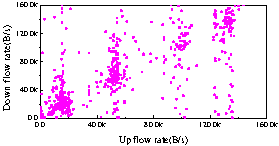
\includegraphics[width=1.8in]{up-down-rate}
	\label{fig:up-down-rate}}
\hspace{1em}%
\subfigure[FCT of upload and download flows.]{
	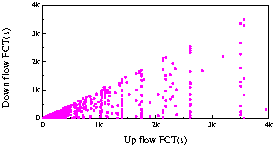
\includegraphics[width=1.8in]{up-down-fct}
	\label{fig:up-down-fct}}
	\hspace{1em}%
\subfigure[The corresponding download flow FCT with upload flow throughput.]{
	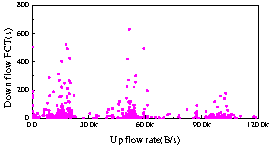
\includegraphics[width=1.8in]{up-rate-down-fct}
	\label{fig:up-rate-down-fct}}
\caption{Relationship between upload and download flows for the same video.}
\label{fig:relationship-up-down} %% label for entire figure
\termspace
\end{figure}


%\begin{figure}[ht]
%	\centering
%	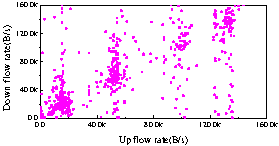
\includegraphics[width=\linewidth]{up-down-rate}
%	\caption{The corresponding rate of upload and download flows.}
%	\label{fig:up-down-rate}
%	\termspace
%\end{figure}

Figure~\ref{fig:up-down-fct} shows the FCT of upload and download follows. From the figure we can find that the points spread below the $y = x$ line, indicating that the FCT of download flows is shorter than that of upload flow. And we also find that the points spread discretely, which means that the FCT of download flows is independent with that of upload flows. Figure~\ref{fig:up-rate-down-fct} shows the relationship between the FCT of download flows and the throughput of upload flows. Most of the FCT of download flows is shorter than 200s. The throughput of upload flows is irrelevant with the FCT of download flows. Even when the throughput of upload flows grows to 100KB/s, most of the FCT of download flows is under 50s, nearly the same as when the throughput of upload flows is about 18KB/s. Figure~\ref{fig:up-down-fct} and Figure~\ref{fig:up-rate-down-fct} confirm that the FCT and throughput of upload flows do not have obvious influence on the FCT of the download flows. So we infer that the content features of the upload video are the key factor that impacts the FCT of download flows. 
%\begin{figure}[ht]
%	\centering
%	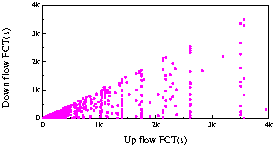
\includegraphics[width=\linewidth]{up-down-fct}
%	\caption{The corresponding flow complete time of upload and download flows.}
%	\label{fig:up-down-fct}
%	\termspace
%\end{figure}

%\begin{figure}[ht]
%	\centering
%	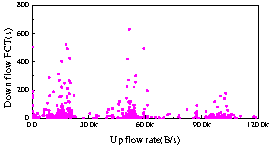
\includegraphics[width=\linewidth]{up-rate-down-fct}
%	\caption{The corresponding download flow FCT with upload flow rate.}
%	\label{fig:up-rate-down-fct}
%	\termspace
%\end{figure}

We also measure the impact of stalls in upload flows on the download flows. We find that 37.2\% of stalls in upload flows will cause stalls in download flows, most of which appear as \emph{resource constraint}, occupying the largest portion of the stalls in download flows. 
%Although we can not match the storage stall with download flows, we think most of the stall in storage flow will also cause \emph{resource constraint} stall in download flows. It is easy to understand as all the stall in upload and storage flows influence the data supply for download flows.